\section{Evaluation} \label{sec:Evaluation}

In dem vorliegenden Kapitel wird kurz die Durchführung der Versuchsreihe beschrieben und die Evaluierung der Ergebnisse des Versuchssystems durchgeführt.
Hierzu werden die Ergebnisse aufbereitet und anhand mehrerer Metriken verglichen.

Das Versuchssystem wird über das Ausführen der \codestyle{main.py}-Datei gestartet (siehe linke Lane im Sequenzdiagramm (Abbildung \ref{fig:sequenzdiagramm-versuchssystem})).
Hier lässt sich spezifizieren, welche der Konfigurationen bei der aktuellen Ausführung analysiert werden sollen, wie man in Zeile~\ref{line:runrange} des Listing~\ref{lst-mainpy} erkennen kann.

\begin{lstlisting}[language=Python,numbers=none,caption=Ausführen einer Versuchsreihe,label=lst-mainpy,escapechar=|]
# load configs from json file
configs = []
with open(os.path.join(os.path.dirname(__file__), "Configs", "configs.json"), "r") as json_file:
    configs = json.load(json_file)

# range for current run
controller = Controller(os.path.join(os.path.dirname(__file__), "results.csv"))
for i in range(0, 20): |\label{line:runrange}|# range for current run
    controller.set_config(configs[i])
    controller.start()
\end{lstlisting}

Da die Analyse von einer Konfiguration im Durchschnitt etwa 35 Minuten dauert, werden die Konfigurationen auf mehrere Geräte aufgeteilt. 
Es kommen insgesamt fünf verschiedene Geräte mit unterschiedlicher Leistung zum Einsatz, die die Konfigurationen blockweise abarbeiten.
Der gesamte Prozess dauert ca. eineinhalb Wochen, wobei zu beachten ist, dass die verwendeten Geräte nicht rund um die Uhr rechnen.
Die Ergebnisse der Analysen werden in CSV-Dateien geschrieben, welche nach dem Beenden der Berechnungen zusammengeführt werden.

Für die Auswertung der Zuordnungsverteilungen aller Konfigurationen des Versuchssystems werden die Ergebnisse zunächst grafisch dargestellt.
Dabei werden in allen Grafiken die Ergebnisse der drei neuronalen Netze pro Konfiguration miteinander verrechnet.
Es werden vier verschiedene Aspekte betrachtet (vgl. Abbildung~\ref{fig:AuswertungVersuchssystem}).
\begin{figure}[H]
    \centering
    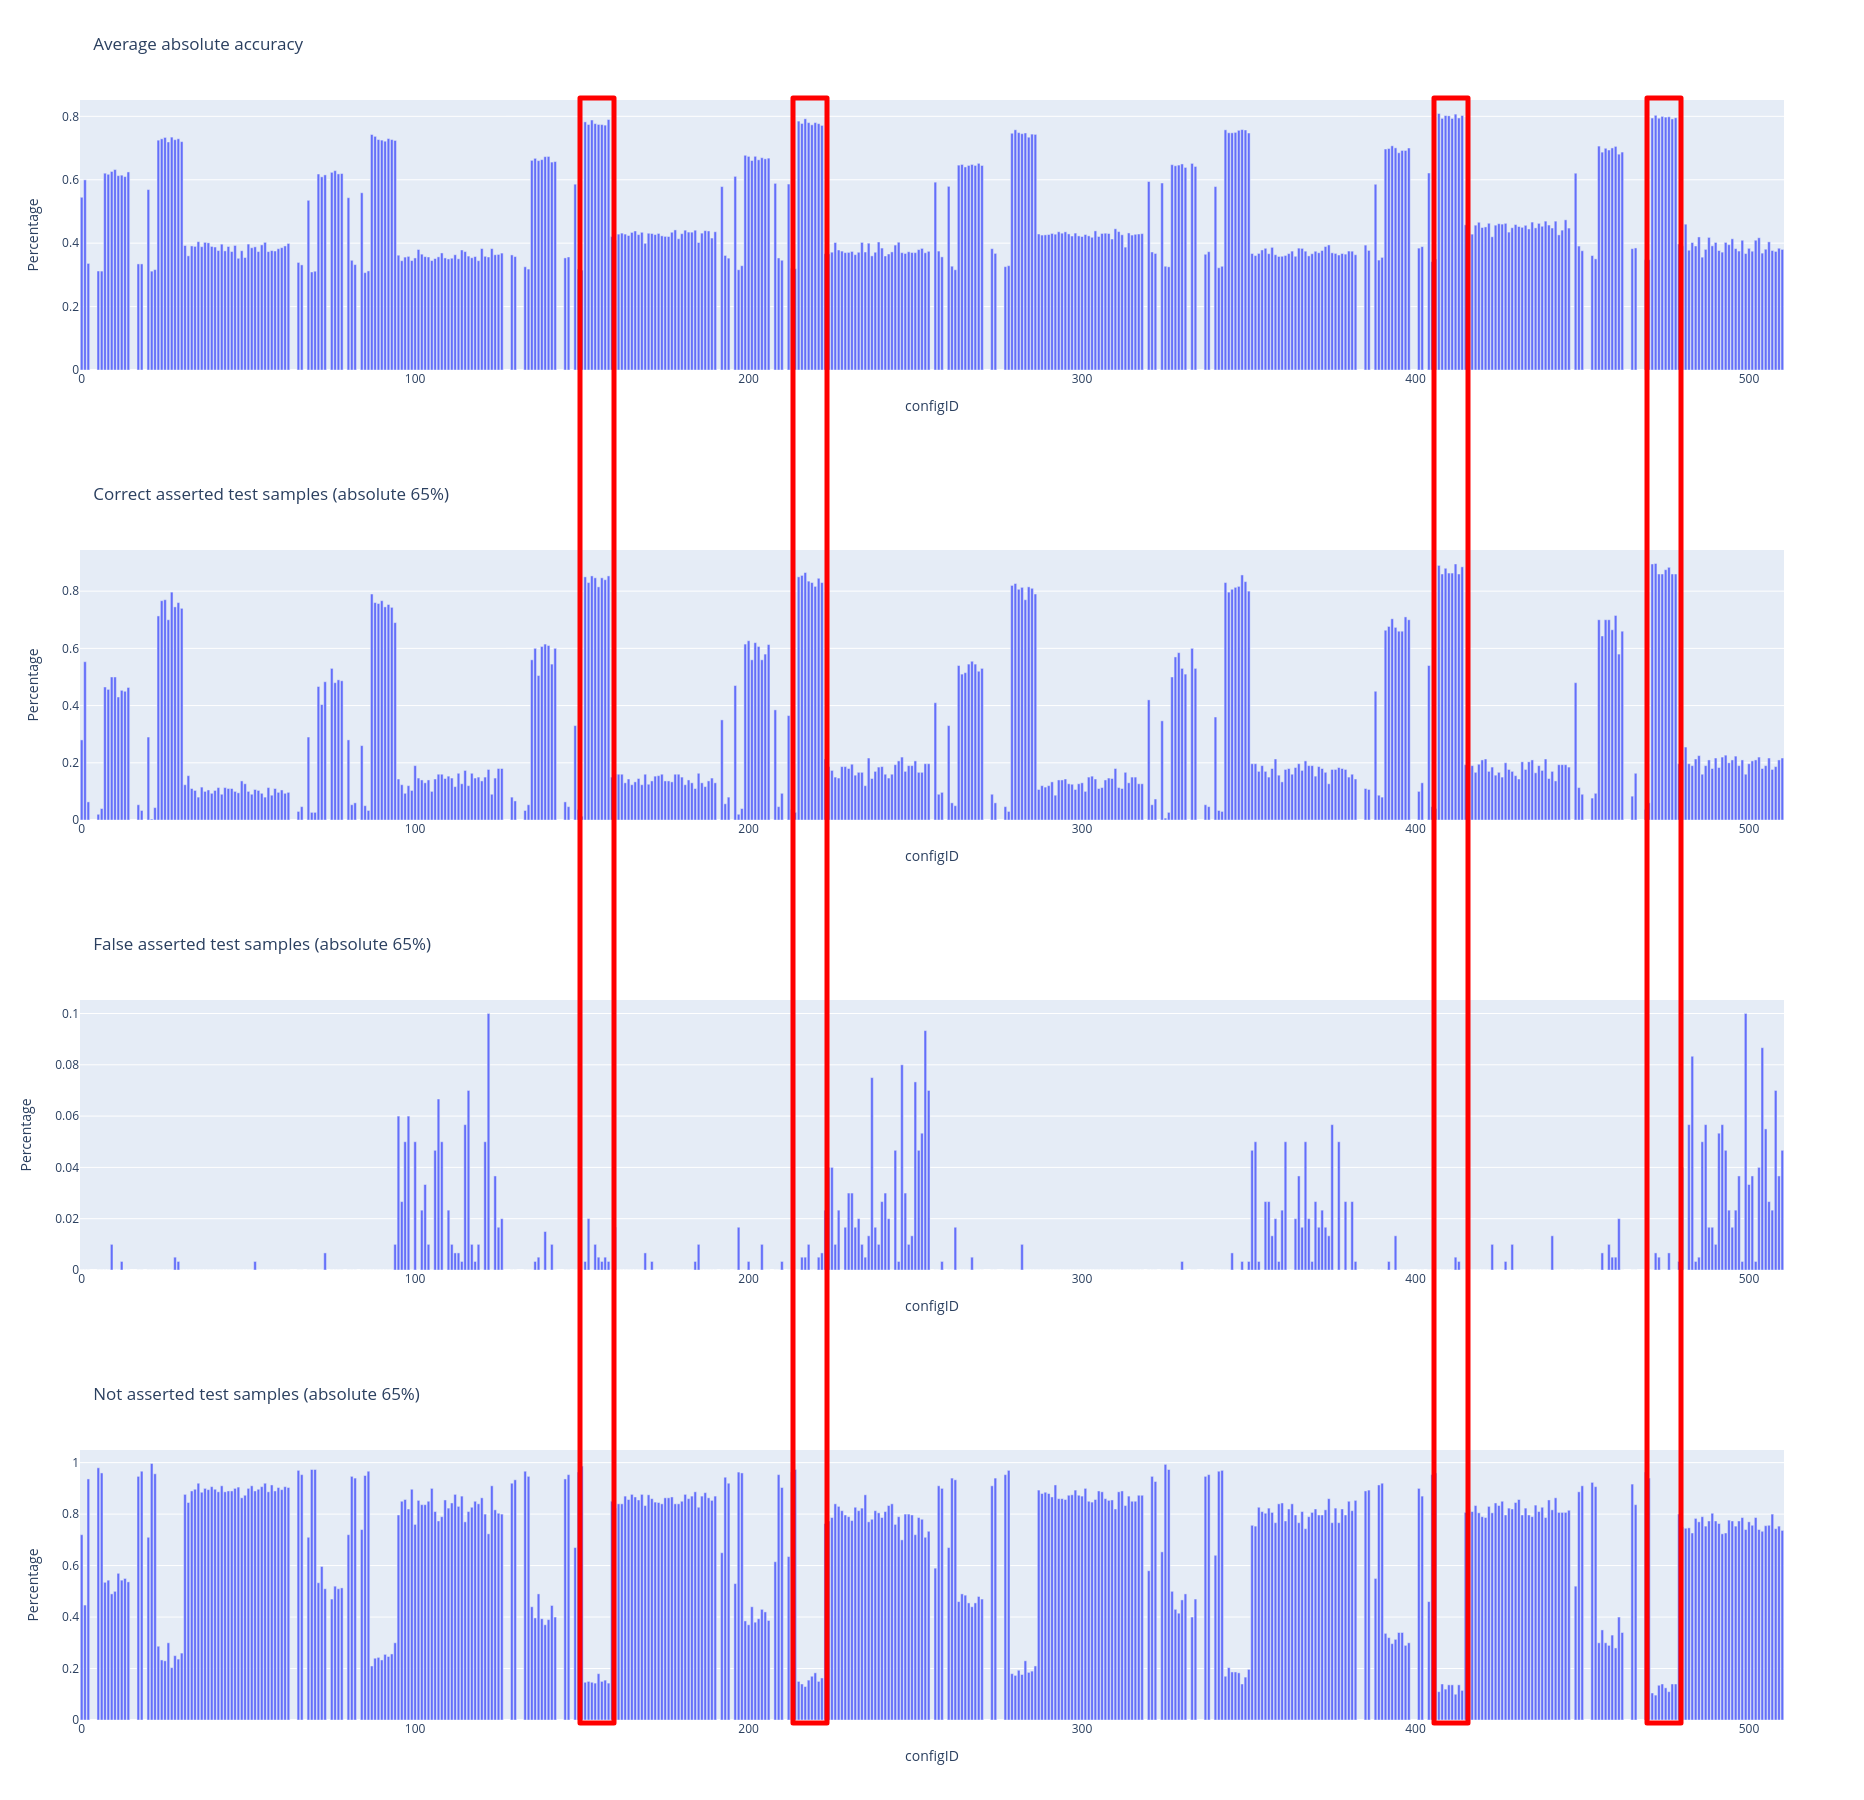
\includegraphics[width=1\textwidth, keepaspectratio]{images/Auswertung.png}
    \caption{Auswertung Versuchssystem}
    \label{fig:AuswertungVersuchssystem}
\end{figure}

Für die durchschnittliche absolute Genauigkeit (erstes Diagramm) werden die Wahrscheinlichkeiten für den zu identifizierenden Benutzer pro Testdatei aufsummiert und der Durchschnitt gebildet.
Eine Genauigkeit von 80 \% entspricht damit der Aussage, dass das neuronale Netz in Kombination mit der jeweiligen Konfiguration dem zu authentifizierenden Benutzer im Durchschnitt 80 \% der Frames der Testdatei zuordnet.

Bereits in dieser Grafik zeigt sich die Bildung von Clustern.
Die besten Konfigurationen erreichen eine Genauigkeit von über 65 \%, weshalb dieser Wert für die folgenden drei Auswertungen verwendet wird.
Hier werden die Testdateien mittels dieses Wertes in die drei Kategorien korrekt zugeteilt, falsch zugeteilt und nicht zugeteilt eingeordnet.

Eine Testdatei gilt als korrekt zugeteilt, wenn dem zu authentifizierenden Benutzer mindestens 65 \% der Frames zugeordnet werden.
Analog gilt die Testdatei als nicht korrekt zugeteilt, wenn einem anderen Benutzer mindestens 65 \% der Frames zugeordnet werden.
Erreicht kein Nutzer mindestens 65 \%, so wird die Testdatei als nicht zugeteilt eingestuft.

Unter Betrachtung der durchschnittlichen absoluten Genauigkeit (zweites Diagramm), sowie der korrekt zugeteilten Testdateien, ergeben sich die vier markierten Cluster als beste Konfigurationen.
Auch in den zwei verbleibenden Kategorien, zeichnen sich diese Konfigurationen vor allem durch eine niedrige Anzahl an nicht zugeordneten Dateien (kleiner 25 \%), sowie falsch zugeordneter Dateien (kleiner 2 \%) aus.

Die Bildung der Cluster ist dabei auf die Art und Weise wie die Konfigurationen erzeugt werden zurückzuführen.
Da hier eine bestimmte Systematik vorliegt, enthalten diese Cluster jeweils ähnliche Feature-Kombinationen, wobei die für die Ergebnisse relevanten Features in jeder Konfiguration vorhanden sind.
In den rot markierten Clustern sind dies \ac{MFCC} und \ac{dMFCC} Features.

In einer detaillierteren Analyse im Direktvergleich ergeben sich die in Listing~\ref{ergebnisOutput} dargestellten Konfigurationen als beste Kombinationen:
\begin{lstlisting}[language=JavaScript,numbers=none,caption=Auswertung der Konfigurationen,label=ergebnisOutput]
id: 472 | average_absolute_accuracy: 0.8033 | lpc: 0 | mfcc: 20 | lpcc:  0 | delta_mfcc: 13
id: 474 | average_absolute_accuracy: 0.8015 | lpc: 0 | mfcc: 20 | lpcc: 13 | delta_mfcc: 13
id: 410 | average_absolute_accuracy: 0.8015 | lpc: 0 | mfcc: 20 | lpcc: 13 | delta_mfcc: 13
id: 408 | average_absolute_accuracy: 0.7989 | lpc: 0 | mfcc: 20 | lpcc:  0 | delta_mfcc: 13
id: 414 | average_absolute_accuracy: 0.7986 | lpc: 0 | mfcc: 20 | lpcc: 13 | delta_mfcc: 13
\end{lstlisting}

Die Evaluation ergibt somit, dass die Konfiguration mit der ID 472 die besten Ergebnisse erzielt.
Dabei werden 1500 Frames bei einer Frame-Größe von 600 Samples generiert.
Daraufhin werden 20 \ac{MFCC} Koeffizienten, sowie 13 \ac{dMFCC} Koeffizienten pro Frame erzeugt, welche durch das neuronale Netz ausgewertet werden.
\ac{LPC} und \ac{LPCC} zeigen in den ausgewählten Konfigurationen keinen signifikanten Mehrwert, weshalb diese nicht verwendet werden.

In einem weiteren Schritt wurden basierend auf der Konfiguration 472 weitere Konfigurationen erstellt, um weitere Untersuchungen durchzuführen.
Diese sind in der Tabelle \ref{table:additionalKonfigs} dargestellt.
\begin{table}[H]
    \centering
    \begin{tabular}{l|l|l|l|l}
    ID  & Anzahl Frames & Länge Frames & \ac{MFCC} & \ac{dMFCC} \\ \hline
    511 & 20000         & 600          & 20        & 13     \\ \hline
    512 & 15000         & 800          & 20        & 13     \\ \hline
    513 & 15000         & 600          & 27        & 13     \\ \hline
    514 & 20000         & 800          & 20        & 13     \\ \hline
    515 & 20000         & 600          & 27        & 13     \\ \hline
    516 & 15000         & 800          & 27        & 13    
    \end{tabular}
    \caption{Zusätzliche Konfigurationen}
    \label{table:additionalKonfigs}
\end{table}\noindent
Die vorliegenden Konfigurationen wurden mithilfe desselben Verfahrens ausgewertet, wie die Konfigurationen zuvor.
Die Untersuchungen der Ergebnisse dieser Konfigurationen zeigen minimale Verbesserungen, die auf die erhöhte Datenmenge zurückzuführen sind.
Da diese Verbesserungen im Verhältnis zur steigenden Rechenzeit minimal sind, werden diese nicht weiter verfolgt.
Somit steht die Konfiguration \textbf{472} aus dem vorherigen Durchlauf als finale Kombination fest.

% TODO Auswertung einfügen.